\tableofcontents
\newpage

\hypertarget{symmetric-encryption}{%
\section{Symmetric encryption}\label{symmetric-encryption}}

\textbf{Kerkhoffs Principle}: The security of a system should only
depend on whether the actual key is secret, not on the system itself.
The whole system is assumed to be public. No ``Security by obscurity''.

\hypertarget{scenario-1}{%
\subsection{Scenario 1}\label{scenario-1}}

\textbf{One message with constant length}

\hypertarget{cryptosystems}{%
\subsubsection{Cryptosystems}\label{cryptosystems}}

A cryptosystem is a tuple \(\mathcal{S} = (X, K, Y, e, d)\) with

\begin{itemize}
\tightlist
\item
  X: set of plaintexts
\item
  K: finite set of keys
\item
  Y: set of ciphertexts
\item
  e: encryption function
\item
  d: decryption function
\end{itemize}

Perfect correctness:
\tab\tab \(d(e(x, k), k) \quad \forall x \in X, k \in K\)

No unnecessary ciphertexts: \tab \(Y = \{e(x,k) | x \in X, k \in K\}\)

\hypertarget{vernam-system}{%
\subsubsection{Vernam system}\label{vernam-system}}

The Vernam cryptosystem of length \(l\) is defined as
\((\{0, 1\}^l, \{0, 1\}^l, \{0, 1\}^l, e, d)\) where

\(e(x, k) = x \oplus k\) and \(d(y, k) = y \oplus k\).

A vernam system of length \(l>0\) provides perfect secrecy for every
uniform \(P_K\). It is the perfect system for Scenario 1.

\hypertarget{perfect-secrecy}{%
\subsubsection{Perfect Secrecy}\label{perfect-secrecy}}

A cryptosystem with key distribution \(\mathcal{V} = \mathcal{S}[P_k]\)
provides perfect secrecy if for all plaintext distributions \(P_X\), the
probability of every plaintext remains the same after the ciphertext is
seen, i.e.: \[P(x) = P(x | y) \quad \forall x \in X, y \in Y, P(y) > 0\]

\textbf{Example Proof}:

We need to show the criteria above for all plaintext distributions
\(P_X\). Therefore we use variable probabilities for the plaintexts
\(P_X(a) = p, P_X(b) = 1-p\) (for 2 plaintexts, else \(p_1, ..., p_n\)).

\begin{minipage}{.35\linewidth}
    \centering
    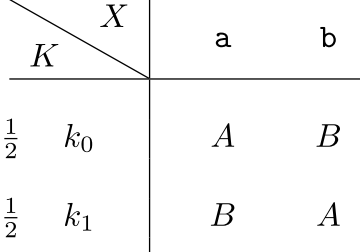
\includegraphics[width=\linewidth]{img/perfect_secrecy_example}
\end{minipage}
\begin{minipage}{.63\linewidth}
    \begin{align*}
        P(a | A) &= \frac{P(a, A)}{P(A)} &= \frac{\frac{1}{2} * p}{\frac{1}{2} * p + \frac{1}{2} * (1-p)} &= p = P(a)\\
        P(a | B) &= \frac{P(a, B)}{P(B)} &= \frac{\frac{1}{2} * p}{\frac{1}{2} * p + \frac{1}{2} * (1-p)} &= p = P(a)\\
        P(b | A) &= \frac{P(b, A)}{P(A)} &= \frac{\frac{1}{2} * (1-p)}{\frac{1}{2} * (1-p) + \frac{1}{2} * p} &= 1-p = P(b)\\
        P(b | B) &= \frac{P(b, B)}{P(B)} &= \frac{\frac{1}{2} * (1-p)}{\frac{1}{2} * (1-p) + \frac{1}{2} * p} &= 1-p = P(b)
    \end{align*}
\end{minipage}
\newline

\textbf{Theorem}:

Let \(\mathcal{S} = (X,K,Y,e,d)\) be a cryptosystem providing perfect
secrecy, then it holds \(|K| \geq |Y| \geq |X|\).

\textbf{Shannons Theorem}:

Let \(\mathcal{V} = \mathcal{S}[P_k]\) be a cryptosystem with key
distribution \(P_K\) and \(|K| = |Y| = |X|\). The system provides
perfect secrecy if and only if

\begin{enumerate}
\def\labelenumi{\arabic{enumi}.}
\tightlist
\item
  \(P_K\) is a uniform distribution
\item
  \(\forall x \in X, y \in Y \exists k \in K \text{ with } e(x, k) = y\)
  (There must be a key for every plaintext/ciphertext pair)
\end{enumerate}

\hypertarget{scenario-2}{%
\subsection{Scenario 2}\label{scenario-2}}

\textbf{Multiple messages with constant length, no repetition}

\hypertarget{vernam-in-scenario-2}{%
\subsubsection{Vernam in Scenario 2}\label{vernam-in-scenario-2}}

Vernam is not a secure cryptosystem anymore, since from 2 ciphertexts,
Eve can learn non-trivial information about the plaintexts:
\[y_0 \oplus y_1 = x_0 \oplus k \oplus x_1 \oplus k = x_0 \oplus x_1\]

Also with 1 plaintext-ciphertext pair (CPA), the key can be calculated
as \(k = x \oplus y\).

\hypertarget{substitution-cryptosystem}{%
\subsubsection{Substitution
Cryptosystem}\label{substitution-cryptosystem}}

Let \(X\) be a non-empty finite set. A substitution cryptosystem over X
is a tuple \((X, P_X, X, e, d)\) where \(P_X\) is the set of all
permutations of \(X\).
\[e(x, \pi) = \pi(x) \quad d(y, \pi) = \pi^{-1}(y) \quad \forall x,y \in X, \pi \in P_X\]

Substitution cryptosystems provide ``perfect security'' in scenario 2,
but they are impractical because the substitution table (\(\pi\)) has a
size of \(2^l * l\).

\hypertarget{l-block-cipher}{%
\subsubsection{\texorpdfstring{\(l\)-Block
Cipher}{l-Block Cipher}}\label{l-block-cipher}}

Let \(l : \mathbb{N} \rightarrow \mathbb{N}\) be a polynomial. An
\(l\)-block cipher \(B\) is a cryptosystem of the form

\(\bigg(\{0,1\}^{l(\eta)}_{\eta \in \mathbb{N}},\; Gen(1^\eta),\; \{0,1\}^{l(\eta)}_{\eta \in \mathbb{N}},\; E,\; D \bigg)\)
or simplified:
\(\bigg(\{0,1\}^l,\; Gen(1^\eta),\; \{0,1\}^l,\; E,\; D \bigg)\)

\hypertarget{substitution-permutation-cryptosystem-spcs}{%
\subsubsection{Substitution-Permutation Cryptosystem
(SPCS)}\label{substitution-permutation-cryptosystem-spcs}}

\textbf{Notation}:

\begin{itemize}
\tightlist
\item
  plaintexts are split into \(m\) words with length \(n\) with
  \(l = m*n\), \(x^{(i)}\) denotes the \(i\)'th word
\item
  \([r] = \{0, 1, ..., r-1\}\)
\item
  \(\beta \in \mathcal{P}_{[l]}\), then \(x^\beta(i) = x(\beta(i))\)
\end{itemize}

\textbf{General Principle}: Over \(r\) rounds, (round) key additions,
word substitutions and bit permutations are applied, including an
initial step that just applies key addition and shortened last round
without bit permutation.

\begin{minipage}{.6\linewidth}
    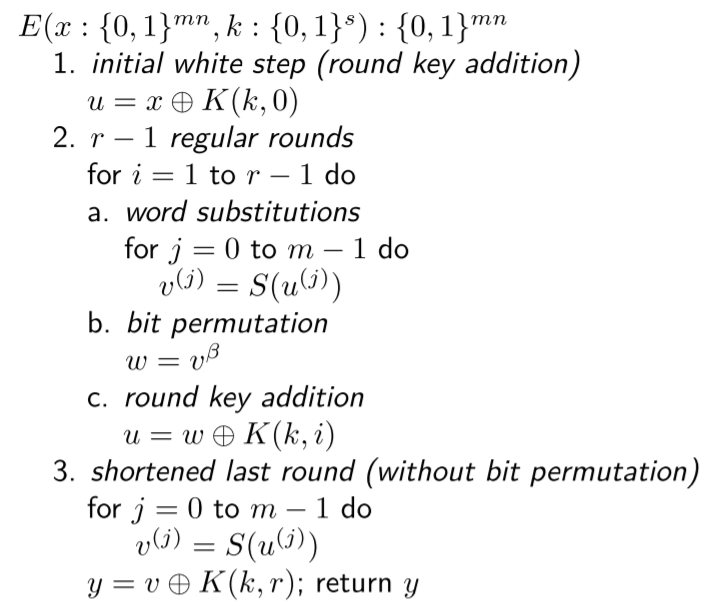
\includegraphics[width=\linewidth]{img/spcs}
\end{minipage}
\begin{minipage}{.35\linewidth}
    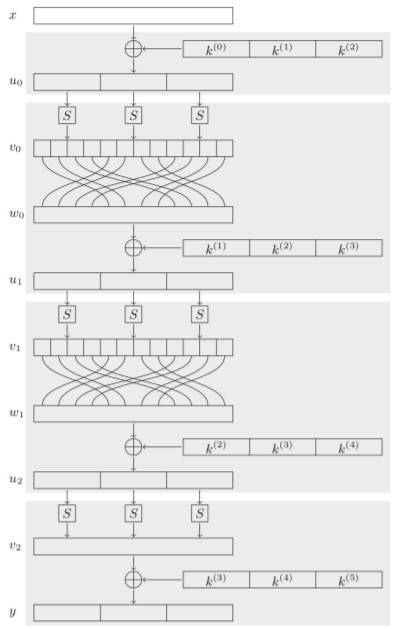
\includegraphics[width=\linewidth]{img/spcs_vis}
\end{minipage}

\textbf{Known Attacks}:

\begin{itemize}
\tightlist
\item
  Brute Force Attack
\item
  Linear Cryptanalysis
\item
  Differential Cryptanalysis
\end{itemize}

\textbf{Linear Cryptanalysis}:

\begin{itemize}
\tightlist
\item
  Relies on a set \(T\) of plaintext-ciphertext pairs
\item
  Instead of brute forcing the whole key, get small parts of the key at
  a time
\item
  Exploit linear dependencies
\end{itemize}

\textbf{AES (Advanced encryption standard)}: basically SPCS with
modifications

\hypertarget{algorithmic-security-of-block-ciphers}{%
\subsubsection{Algorithmic Security of Block
Ciphers}\label{algorithmic-security-of-block-ciphers}}

\begin{minipage}{.55\linewidth}

We consider a block cipher secure if it is almost as good as a
substitution cryptosystem w.r.t. resource-bound adversaries. Therefore
no adversary \(U\) should be able to distinguish BCS and SCS. Formally,
we use the BCS for \(b=1\) (real world) and the SCS for \(b=0\) (random
world) in the security game.

The winning probability is \(Pr[\mathbb{E}(1^n) = 1]\). Since a random
guesser already has a probability of \(0.5\), the advantage is
normalized.

\end{minipage}\hfill
\begin{minipage}{.4\linewidth}

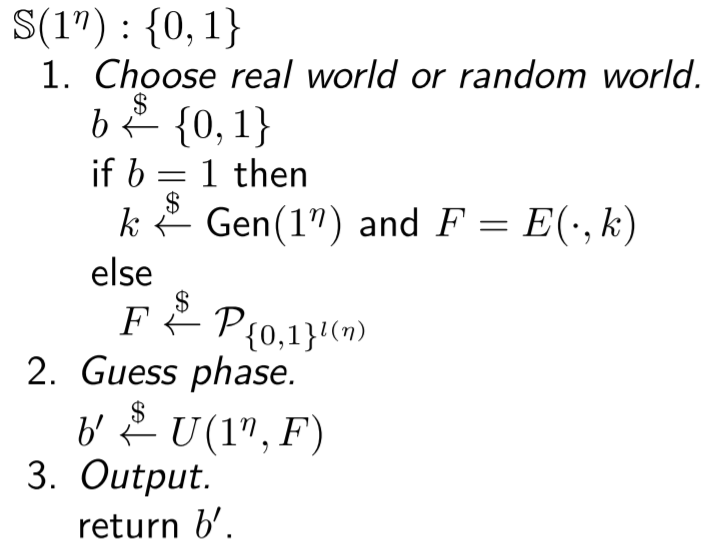
\includegraphics{img/BC_SG.png}

\end{minipage}

\begin{align*}
    Adv_{U, B}(\eta) &= 2 * \bigg( Pr[\mathbb{E}_U^B(1^\eta) = 1] - \frac{1}{2} \bigg) \in [-1, 1]
    &suc_{U, B}(\eta) = Pr[\mathbb{S}_U^B\langle b=1\rangle (1^\eta) = 1]\\
    Adv_{U, B}(\eta) &= suc_{U, B}(\eta) - fail_{U, B}(\eta)
    &fail_{U, B}(\eta) = Pr[\mathbb{S}_U^B\langle b=0\rangle (1^\eta) = 1]  
\end{align*}

\hypertarget{prpprf-switching-lemma}{%
\subsubsection{PRP/PRF Switching Lemma}\label{prpprf-switching-lemma}}

Since substitution cryptosystems cannot be distinguished from (secure)
\(l\)-Block cryptosystems, we can see \(l\)-Block cryptosystems as
pseudo-random permutations (PRP). Anyway, for proving purposes, it can
be easier to see them as pseudo-random functions. The PRP/PRF Switching
Lemma says, that we can use them interchangeably, since the difference
of advantages is negligible:

Let \(B\) be an \(l\)-block cipher and \(U\) be an \(l\)-distinguisher
with runtime bound \(q(\eta)\) where q is a positive polynomial and
\(\eta \in \mathbb{N}\). Then the following holds true:
\[|Adv^{PRP}_{U,B}(\eta) - Adv^{PRF}_{U,B}(\eta)| \leq \frac{q(\eta)^2}{2^{l(\eta)+1}}\]

\hypertarget{scenario-3}{%
\subsection{Scenario 3}\label{scenario-3}}

\textbf{Arbitrary messages with any length (possibly with repetition)}

\hypertarget{symmetric-encryption-scheme}{%
\subsubsection{Symmetric Encryption
Scheme}\label{symmetric-encryption-scheme}}

A symmetric encryption scheme is a tuple \(S = (Gen(^\eta), E, D)\) with

\begin{itemize}
\tightlist
\item
  security parameter \(\eta\)
\item
  ppt key generation algorithm \(Gen(1^\eta)\)
\item
  ppt encryption algorithm \(E(x: \{0, 1\}^*, k: K) : \{0,1\}^*\)
\item
  dpt decryption algorithm \(D(y: \{0,1\}^*, k: K) : \{0,1\}^*\)
\item
  and \(D(E(x, k), k) = x\)
\end{itemize}

E cannot be deterministic, because else we wouldn't be able to send the
same message multiple times, i.e.~the same plaintext encrypted under the
same key should result in a different ciphertext (with a high
probability).

\hypertarget{encryption-schemes-from-stream-ciphers}{%
\subsubsection{Encryption Schemes from Stream
Ciphers}\label{encryption-schemes-from-stream-ciphers}}

\textbf{Idea}: Vernam is safe if we use every key just once. So using
the key as seed of a random number generator, that generates a stream of
random numbers, enables the usage of the vernam system for arbitrarily
long messages.

\hypertarget{number-generator}{%
\paragraph{Number generator}\label{number-generator}}

A number generator (NG) is a dpt algorithm of the Form
\(G : (s: \{0,1\}^\eta) : \{0,1\}^{p(\eta)}\) where \(p\) is the
expansion factor.

\hypertarget{prng-distinguisher}{%
\paragraph{PRNG-Distinguisher}\label{prng-distinguisher}}

TODO

\hypertarget{encryption-schemes-from-block-ciphers}{%
\subsubsection{Encryption Schemes from Block
Ciphers}\label{encryption-schemes-from-block-ciphers}}

\hypertarget{ecb-mode}{%
\paragraph{ECB Mode}\label{ecb-mode}}

\textbf{Idea}: Split the message in blocks of constant length and
encrypt each block under the given key using the underlying block
cipher.

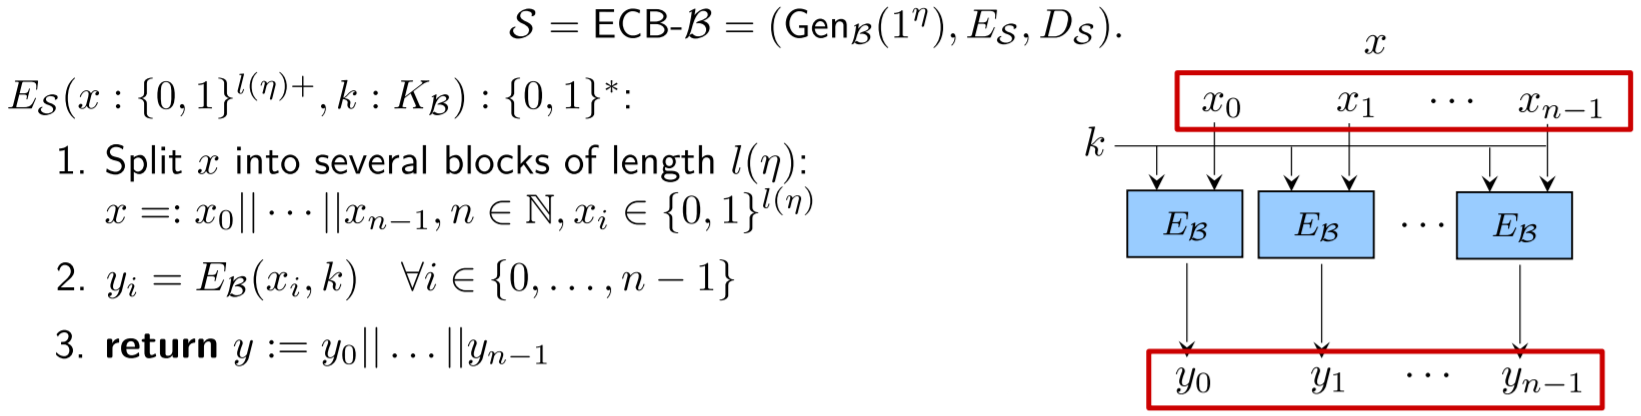
\includegraphics[width=\linewidth]{img/ecb-mode}

\textbf{Security}: It's not secure, since the ciphertext carries
non-trivial information about the plaintext:
\(\text{for } y = y_0 || y_1\text{, then } y_0 = y_1 \text{ if } x_0 = x_1\).

\hypertarget{cbc-mode}{%
\paragraph{CBC Mode}\label{cbc-mode}}

\begin{minipage}{.55\linewidth}

\textbf{Idea}: Add and initialization vector \(v\) that is
\texttt{xor}'ed with the plaintext before encrypting. That \(v\) is part
of the key. \newline\newline \textbf{Problem}: Still deterministic, so
every plaintext can be sent just once.

\end{minipage}\hfill
\begin{minipage}{.4\linewidth}
    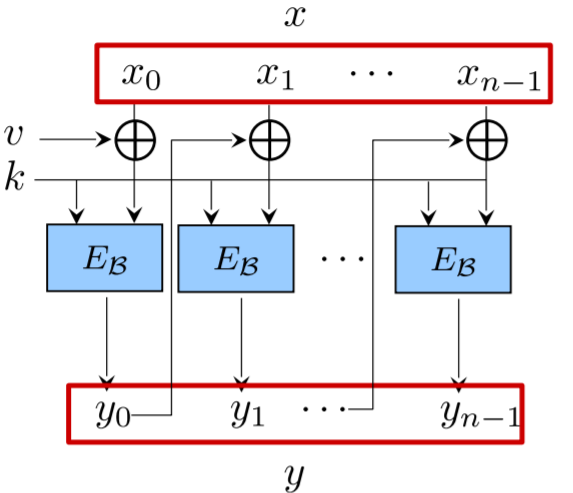
\includegraphics[width=\linewidth]{img/cbc-mode}
\end{minipage}

\hypertarget{r-cbc-mode}{%
\paragraph{R-CBC Mode}\label{r-cbc-mode}}

\begin{minipage}{.55\linewidth}

\textbf{Idea}: To solve the issues of CBC-Mode, R-CBC moves the
initialization vector \(v\) out of the key and generates a random one
while decryption. The vector is appended as first block of the
ciphertext to enable decryption. \newline\newline \textbf{Security}: Its
secure if the underlying block cipher is secure.

\end{minipage}\hfill
\begin{minipage}{.4\linewidth}
    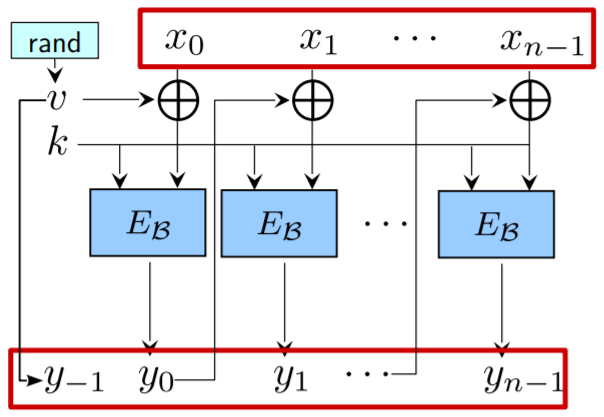
\includegraphics[width=\linewidth]{img/rcbc-mode}
\end{minipage}

\hypertarget{r-ctr-mode}{%
\paragraph{R-CTR Mode}\label{r-ctr-mode}}

\begin{minipage}{.55\linewidth}

\textbf{Idea}: Alternative to R-CBC. Generate a random number \(r\)
(comparable to \(v\) of R-CBC), encrypt this random number under the key
and xor it with the plaintext. The counter is increased by 1 for each
block. The counter \(r\) is appended as first block of \(y\) to enable
decryption. \newline\newline \textbf{Security}: Its secure if the
underlying block cipher is secure.

\end{minipage}\hfill
\begin{minipage}{.4\linewidth}
    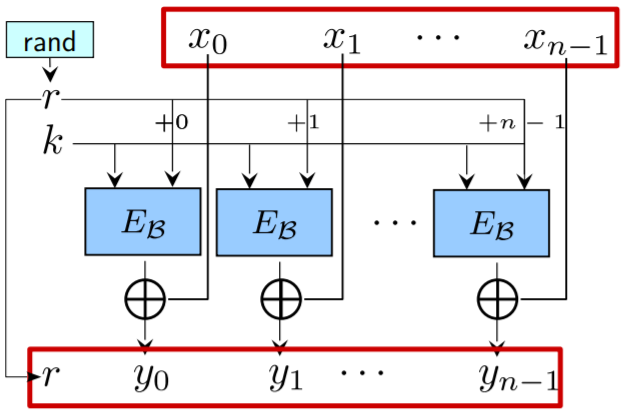
\includegraphics[width=\linewidth]{img/rctr-mode}
\end{minipage}

\hypertarget{cpa-security}{%
\subsubsection{CPA-Security}\label{cpa-security}}

\begin{minipage}{.62\linewidth}

\textbf{CPA}: Chosen-Plaintext-Attack \newline\newline \textbf{Game}:
Adversary \(A\) consists of finder \(AF\) and guesser \(AG\). The finder
chooses 2 plaintexts \(z_0, z_1\). One of them is encrypted. The guesser
has to determine which of them is the corresponding plaintext.
\newline\newline Advantage, success and failure are defined as for block
ciphers.

\end{minipage}\hfill
\begin{minipage}{.35\linewidth}
    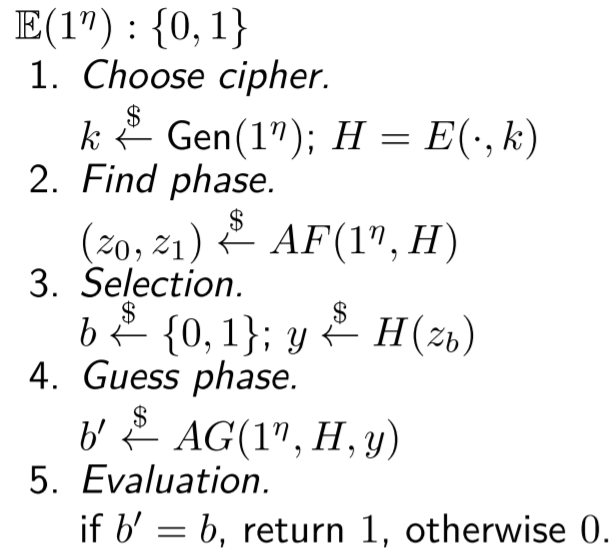
\includegraphics[width=\linewidth]{img/cpa}
\end{minipage}

\hypertarget{cca-security}{%
\subsubsection{CCA-Security}\label{cca-security}}

\begin{minipage}{.62\linewidth}

\textbf{CCA}: Chosen-Ciphertext-Attack \newline\newline \textbf{Game}:
In addition to the encryption oracle \(H\) from the CPA-game, the
adversary also gets a decryption oracle \(H^{-1}\). \newline\newline
Advantage, success and failure are defined as for block ciphers.

\end{minipage}\hfill
\begin{minipage}{.35\linewidth}
    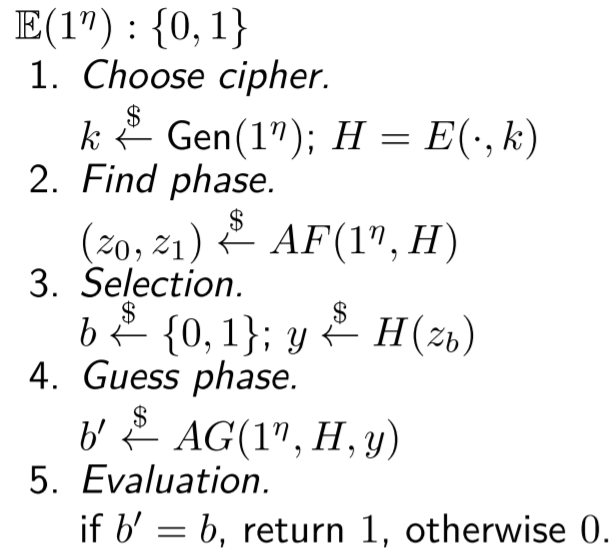
\includegraphics[width=\linewidth]{img/cpa}
\end{minipage}

\hypertarget{vaudenays-padding-attack}{%
\subsubsection{Vaudenay's Padding
Attack}\label{vaudenays-padding-attack}}

\begin{itemize}
\tightlist
\item
  TODO
\end{itemize}

\hypertarget{number-theory}{%
\section{Number Theory}\label{number-theory}}

\hypertarget{fundamental-theorem-of-arithmetic}{%
\subsection{Fundamental Theorem of
Arithmetic}\label{fundamental-theorem-of-arithmetic}}

Every natural number \(n \in \mathbb{N}, n \geq 2\) has exactly one
combination of prime factors.
\[n = p_1 * \dots * p_k \quad \text{with} k \leq log(n)\]

\hypertarget{modulo}{%
\subsection{Modulo}\label{modulo}}

Let \(n \in \mathbb{N}\backslash \{0\}, a \in \mathbb{Z}\). Then
\(\exists !q \in \mathbb{Z}, r \in \{0, \dots, n-1\}\) such that
\(a = n*q + r\).
\[a \text{ div } n := q  \quad\quad\text{and}\quad\quad a \text{ mod } n := r\]

\hypertarget{mathbbz_n}{%
\subsection{\texorpdfstring{\(\mathbb{Z}_n\)}{\textbackslash{}mathbb\{Z\}\_n}}\label{mathbbz_n}}

Let \(n \geq 1\). We define the set
\(\mathbb{Z}_n := \{0, \dots, n-1\}\) of remainders of divisions by
\(n\). Let \(a,b \in \mathbb{Z}_n\), then
\[a +_n b := (a + b) \text{ mod } n \quad\quad\text{and}\quad\quad a *_n b := (a * b) \text{ mod } n\]

\hypertarget{group}{%
\subsection{Group}\label{group}}

A tuple \((\mathcal{G}, \cdot)\) is called group if \(\mathcal{G}\) is a
non-empty set and
\(\cdot : \mathcal{G} \times \mathcal{G} \rightarrow \mathcal{G}\) is a
function such that:

\begin{itemize}
\tightlist
\item
  \((x \cdot y) \cdot z = x \cdot (y \cdot z) \quad\forall x,y,z \in \mathcal{G}\)
  \tab\tab (associativity)
\item
  \(\exists e \in \mathcal{G} : e \cdot x = x \cdot e = x \quad \forall x \in \mathcal{G}\)
  \tab\tab (neutral element)
\item
  \(\forall x \in \mathcal{G} \exists x^{-1} \in \mathcal{G} : x \cdot x^{-1} = e\)
  \tab\tab (inverse element)
\end{itemize}

The \emph{order} of a group is the number of elements in
\(\mathcal{G}\).

The exponentiation is defined as usual. For a finite group
\((\mathcal{G}, \cdot)\) with order \(n\) and neutral element \(e\), the
following holds true:
\[ g^n = e \quad\quad\text{and}\quad\quad g^a = g^{a \text{ mod } n}\]

\hypertarget{ring}{%
\subsection{Ring}\label{ring}}

A Ring is the tuple \((\mathcal{R}, +, \cdot)\) if \((\mathcal{R}, +)\)
is an abelian (commutative) group and the function
\(\cdot : \mathcal{R} \times \mathcal{R} \rightarrow \mathcal{R}\) is
associative, distributive and has a neutral element.

The set of invertible elements in \(\mathcal{R}\) is denoted by
\(\mathcal{R}^*\). The tuple \((\mathcal{R}^*, \cdot)\) is an abelian
group called group of units.

\hypertarget{greatest-common-divisor}{%
\subsection{Greatest common divisor}\label{greatest-common-divisor}}

We say \(a \text{ divides } b\) or \(a | b\) if
\(\exists c \in \mathbb{Z} : b = c \cdot a\). The greatest common
divisor is definded as
\[gcd(a, b) = max\{c : c | a \text{ and } c | b\} \text{ where } gcd(0,0) := 0\]

The set of invertible elements of \(\mathbb{Z}_n\) can be determined by
the gcd. \[\mathbb{Z}_n^* = \{a \in \mathbb{Z}_n | gcd(a, n) = 1\}\]

\hypertarget{eurlers-totient-function}{%
\subsection{Eurler's Totient Function}\label{eurlers-totient-function}}

Let \(n \geq 2\). The Euler's totient function is defined by
\[\Phi(n) = | \mathbb{Z}_n^* | = (p_0 - 1) \cdot p_0^{\alpha_0 - 1} \dots (p_{r-1} - 1) \cdot p_{r-1}^{\alpha_{r-1} - 1}\]
where \(p_1, \dots, p_{r-1}\) are primes and
\(n = p_0^{\alpha_0} \dots p_{r-1}^{\alpha_{r-1}}\). Let \(p\) be a
prime, then \(\Phi(p) = p - 1\).

It can also be used to calculate the number of generators in a cyclic
group as \(\Phi(n) \text{ where } n = |\mathcal{G}|\).

\hypertarget{euclids-algorithm}{%
\subsection{Euclids Algorithm}\label{euclids-algorithm}}

\begin{minipage}{.3\linewidth}
Algorithm to calculate the gcd. Can be extended to calculate the inverse of an element in $\mathbb{Z}_n^*$.
\end{minipage}\hfill
\begin{minipage}{.65\linewidth}
    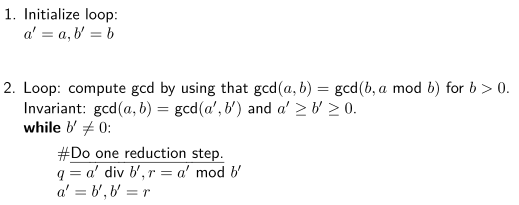
\includegraphics[width=\linewidth]{img/euclid}
\end{minipage}

\hypertarget{fast-exponentiation}{%
\subsection{Fast Exponentiation}\label{fast-exponentiation}}

\begin{minipage}{.7\linewidth}

Algorithm to efficiently compute the exponentiation of a group element.
Let \(\mathcal{G}\) be a group and
\(g \in \mathcal{G}, m \in \mathbb{N}\). It uses the fact, that
\(g^{2k} = (g^k)^2\). Instead of doing \(2k\) multiplications, we can do
\(k + 1\). This is applied recursively to minimize the number of
exponentiations that need to be computed. To make the algorithm work
with any \(k\) (not just powers of \(2\)), we use the binary
representation of the exponent, e.g.
\[13 = 2^0 + 2^2 + 2^3 = (1101)_2 \quad \Rightarrow \quad g^{13} = g^{2^0} \cdot g^{2^2} \cdot g^{2^3}\]

To compute \(g^m\), the algorithm iterates over the bits of \(m\). If
the bit is one, multiply the result with the current factor. In any
case, square the current factor.

The algorithm has a complexity of \(\mathcal{O}(log(m))\).

\end{minipage}\hfill
\begin{minipage}{.25\linewidth}
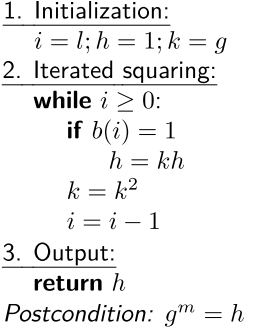
\includegraphics[width=\linewidth]{img/fast_exp}
\end{minipage}

\hypertarget{cyclic-groups}{%
\subsection{Cyclic Groups}\label{cyclic-groups}}

A group \(\mathcal{G}\) is called cyclic, iff
\(\exists g \in \mathcal{G}\) such that
\(\langle g\rangle = \mathcal{G}\).

If \(p = |\mathcal{G}|\) is prime, then \(\mathcal{G}\) is a cyclic
group.

\(\mathbb{Z}_p^*\) is a cyclic group if \(p\) is prime.

\hypertarget{subgroups}{%
\subsubsection{Subgroups}\label{subgroups}}

Let \((\mathcal{G}, \cdot)\) be a finite group and
\(U \subseteq \mathcal{G}\).

\textbf{Definition}: The tuple \((U, \cdot)\) is a subgroup of
\(\mathcal{G}\) iff \(U\) is a group.

\textbf{Lemma}: The tuple \((U, \cdot)\) is a subgroup of
\(\mathcal{G}\) iff \(1 \in U\) and
\(a \cdot b \in U \quad \forall a,b \in U\)

\textbf{Lagranges Theorem}: If \(U\) is a subgroup of \(\mathcal{G}\),
then it holds true that \(|U|\;|\;|\mathcal{G}|\).

\hypertarget{generated-groups-and-generators}{%
\subsubsection{Generated Groups and
Generators}\label{generated-groups-and-generators}}

Let \(\mathcal{G}\) be a group and \(g \in \mathcal{G}\). By
\(\langle g\rangle\) we denote the smallest subgroup of \(\mathcal{G}\)
that contains \(g\).
\[\langle g\rangle = \{1, g, g^{-1}, g^{2}, g^{-2}, \dots\}\quad
\text{ and if $\mathcal{G}$ if inite: }
\langle g\rangle = \{1, g, g^{2}, \dots, g^{|\langle g\rangle| - 1}\}\]
We call \(g\) a generator of \(\mathcal{G}\) if
\(\langle g\rangle = \mathcal{G}\).

\hypertarget{finding-generators}{%
\subsubsection{Finding Generators}\label{finding-generators}}

We find generators for a group by guessing a group element and checking
whether or not it is a generator. This can be evaluated by the equation
\[g^{n/p} \neq 1 \quad \forall \quad p \in P \text{ (prime factors of $n$) and } n = |\mathcal{G}|\]

\begin{minipage}{.35\linewidth}
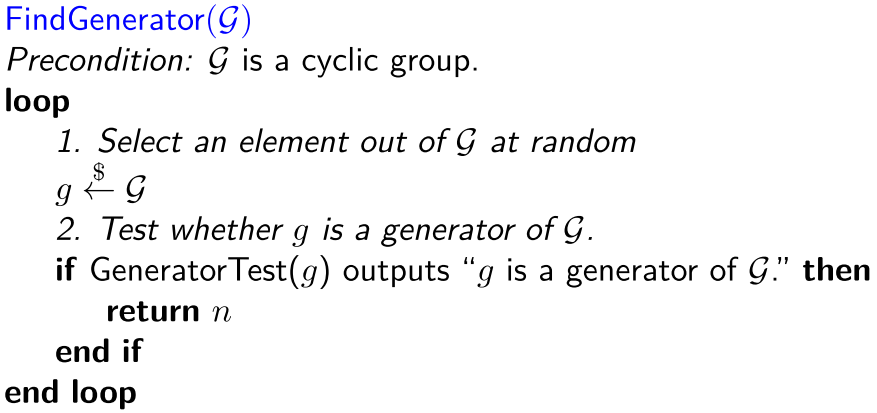
\includegraphics[width=\linewidth]{img/gen_find}
\end{minipage}\hfill
\begin{minipage}{.6\linewidth}
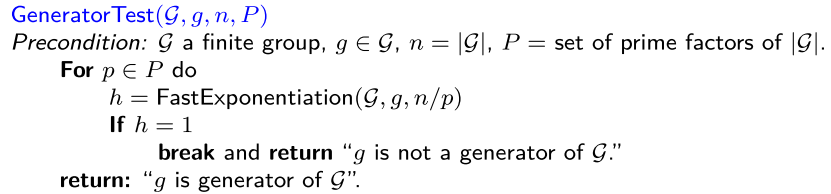
\includegraphics[width=\linewidth]{img/gen_test}
\end{minipage}

This only works, because the probability of finding a generator when
randomly sampling is relatively high, concretely it is upper-bounded by
\(Pr[\langle X_g \rangle = \mathcal{G}] \geq \frac{1}{1+log(n)} \text{ with } X_g \overset{\$}{\leftarrow}\mathcal{G}\).

\hypertarget{quadratic-residues}{%
\subsubsection{Quadratic Residues}\label{quadratic-residues}}

A number \(a \in \mathbb{Z}_n^*\) \emph{quadratic residue modulo \(n\)}
iff there exists \(b \in \mathbb{Z}_n\) such that
\(b^2 \text{ mod } n = a \text{ mod } n\). \(b\) is called root of
\(a\). All quadratic residues modulo n are denoted by \(QR(n)\) and all
elements that are \emph{quadratic nonresidue modulo n} \(QNR(n)\) with
\(\mathbb{Z}_n^* = QR(n) \cup QNR(n)\). For prime \(p\), both sets have
the same order: \[|QR(p)| = |QNR(p)| = \frac{p-1}{2}\]

\hypertarget{eulers-criterion}{%
\subsubsection{Eulers criterion}\label{eulers-criterion}}

Let \(p > 2\) be a prime number, \(a \in \mathbb{Z}\) and
\(e = a^{(p-1)/2} \text{ mod } p\)

\begin{enumerate}
\def\labelenumi{\arabic{enumi}.}
\tightlist
\item
  \(e \in \{0, 1, p-1\}\)
\item
  \(a \text{ mod } p = 0 \Leftrightarrow e = 0\)
\item
  \(a \text{ mod } p \in QR(p) \Leftrightarrow e = 1\)
\item
  \(a \text{ mod } p \in QNR(p) \Leftrightarrow e = -1 \text{ mod } p\)
\end{enumerate}

We also call the criterion \emph{Legendre symbol of \(a\) and \(p\)}
\(L_p(a) = a^{(p-1)/2}\).

\hypertarget{asymmetric-encryption}{%
\section{Asymmetric Encryption}\label{asymmetric-encryption}}

Symmetric encryption is efficient, but requires a key exchange that
makes it impractical for most usecases. Asymmetric encryption works
without key exchange, be splitting the key in public and private.

\hypertarget{asymmetric-encryption-scheme}{%
\subsection{Asymmetric Encryption
Scheme}\label{asymmetric-encryption-scheme}}

As with symmetric encryption, the scheme is a tuple
\(\mathcal{S} = (X, Gen(1^\eta), E, E)\). The key gen algorithm now
outputs a tuple \((k, \hat{k})\) (public, private), the encryption \(E\)
uses the public key \(k\) and decrpytion \(D\) the private key
\(\hat{k}\).

\hypertarget{asymmetric-cpa-security}{%
\subsection{Asymmetric CPA-Security}\label{asymmetric-cpa-security}}

\begin{minipage}{.45\linewidth}
The security game is defined analogously to symmetric encryption. The key is now a tuple and the adversary knows the public key. Advantage, success and failure are defined as for Block Ciphers.
\end{minipage}\hfill
\begin{minipage}{.45\linewidth}
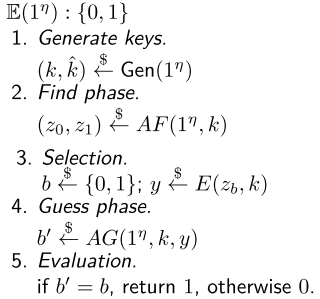
\includegraphics[width=\linewidth]{img/acpa}
\end{minipage}

\hypertarget{rsa}{%
\subsection{RSA}\label{rsa}}

RSA is an asymmetric encryption scheme
\(\mathcal{S}_{RSA} = (X, Gen(1^\eta), E, D)\). It uses the problem of
computing prime factors as oneway function.

\begin{itemize}
\tightlist
\item
  The keygen algorithm randomly selects 2 different primes \(p\) and
  \(q\) of binary length \(\eta\). \begin{alignat*}
  &n = p \cdot q
  &m = (p-1) \cdot (q-1) = \Phi(n)\\
  &e \overset{\$}{\leftarrow}\mathbb{Z}_m^*
  &d = e^{-1} \mod m\\
  &k = ((n,e), (n,d))
  \end{alignat*}
\end{itemize}
